\label{taxi-availability}
\subsubsection{Purpose}

When a taxi driver is ready for a ride, he/she shall be able to notify the system using his mobile phone. With the app he/she can change his status from ``not in service'' to ``in service'' and vice versa.

The city is divided in ``taxi zones''. Taxis can start and stop only inside taxi zones: origins and destinations located outside taxi zones are not allowed by the system.
Each taxi zone is associated with a taxi queue.

When the system receives a status update from the taxi driver, it inserts him/her in the right queue for his/her taxi zone using the information from the taxi GPS if the new status is ``in service'', or it removes him/her from the queue if the new status is ``not in service''.

After a ride, a taxi driver has to notify that the ride is over. The system reinserts the taxi into the right queue.

The queues are FIFO and when a taxi driver refuses a ride, the system moves the taxi to the bottom of the same queue.

When a taxi driver accepts a ride, the system marks the taxi as busy and removes it from the top of the queue.

\subsubsection{Scenario 1}
Ernie gets in his taxi, ready to start his working day. He takes out his phone from his pocket and logs in.

He changes his status in ``in service'', so the system retrieves the GPS position of his taxi, analyses the data and puts the taxi in the right queue.

After thirty minutes the system has an incoming request from his zone. The first taxi on the top of the queue is Ernie's. The system sends a notification to Ernie and waits for a reply.

He receives the request and accepts it. The system pops him from the top of the queue and marks it as busy.

When Ernie finishes the ride, he notifies the system. The system retrieves his new GPS position and re-inserts his taxi in the queue.

\subsubsection{Use case}
The use case for a taxi availability handling is shown in~\autoref{usecase-taxiavailability}.

\begin{table}
\begin{center}
\begin{tabular}{| l | p{0.7\textwidth} |}
\hline
Actor & Taxi driver \\
\hline
Goal & Goal~\ref{g-notify}
\\
\hline
Input condition & Taxi drivers are logged in and change their status to ``in service''.  \\
\hline
Event Flow & \begin{enumerate}
	\item The taxi driver changes his status to ``in service''.
	\item The system enqueues the taxi in the right queue using GPS information.
	\item A new request incomes.
	\item The system chooses the first taxi in the queue and sends the ride request.
	\item The taxi driver can either accept or deny the request; if he denies it, the request is forwarded to the next taxi driver in the queue, and so on.
	\item When a taxi driver accepts the request, the system dequeues the taxi and marks it as busy.
	\item The taxi driver reaches the location.
	\item The taxi driver notifies that the passenger is on board.
	\item When the ride is completed, the taxi driver notifies it to the system.
	\item The system enqueues the taxi in the right queue using GPS data.
	\item The taxi driver changes his status to ``not in service''.
	\item The system dequeues the taxi.
\end{enumerate}
\\
\hline
Output condition & The driver changes is no longer in service and gets dequeued. \\
\hline
Exception & No taxi is available in the passenger's zone. \\
\hline
\end{tabular}
\end{center}
\caption{Use case for taxi availability handling.}
\label{usecase-taxiavailability}
\end{table}

\subsubsection{Response sequence}
The statechart representing the taxi driver's possible statuses is represented in~\autoref{fig:statechart_taxidriver}.
\begin{figure}
	\begin{center}
	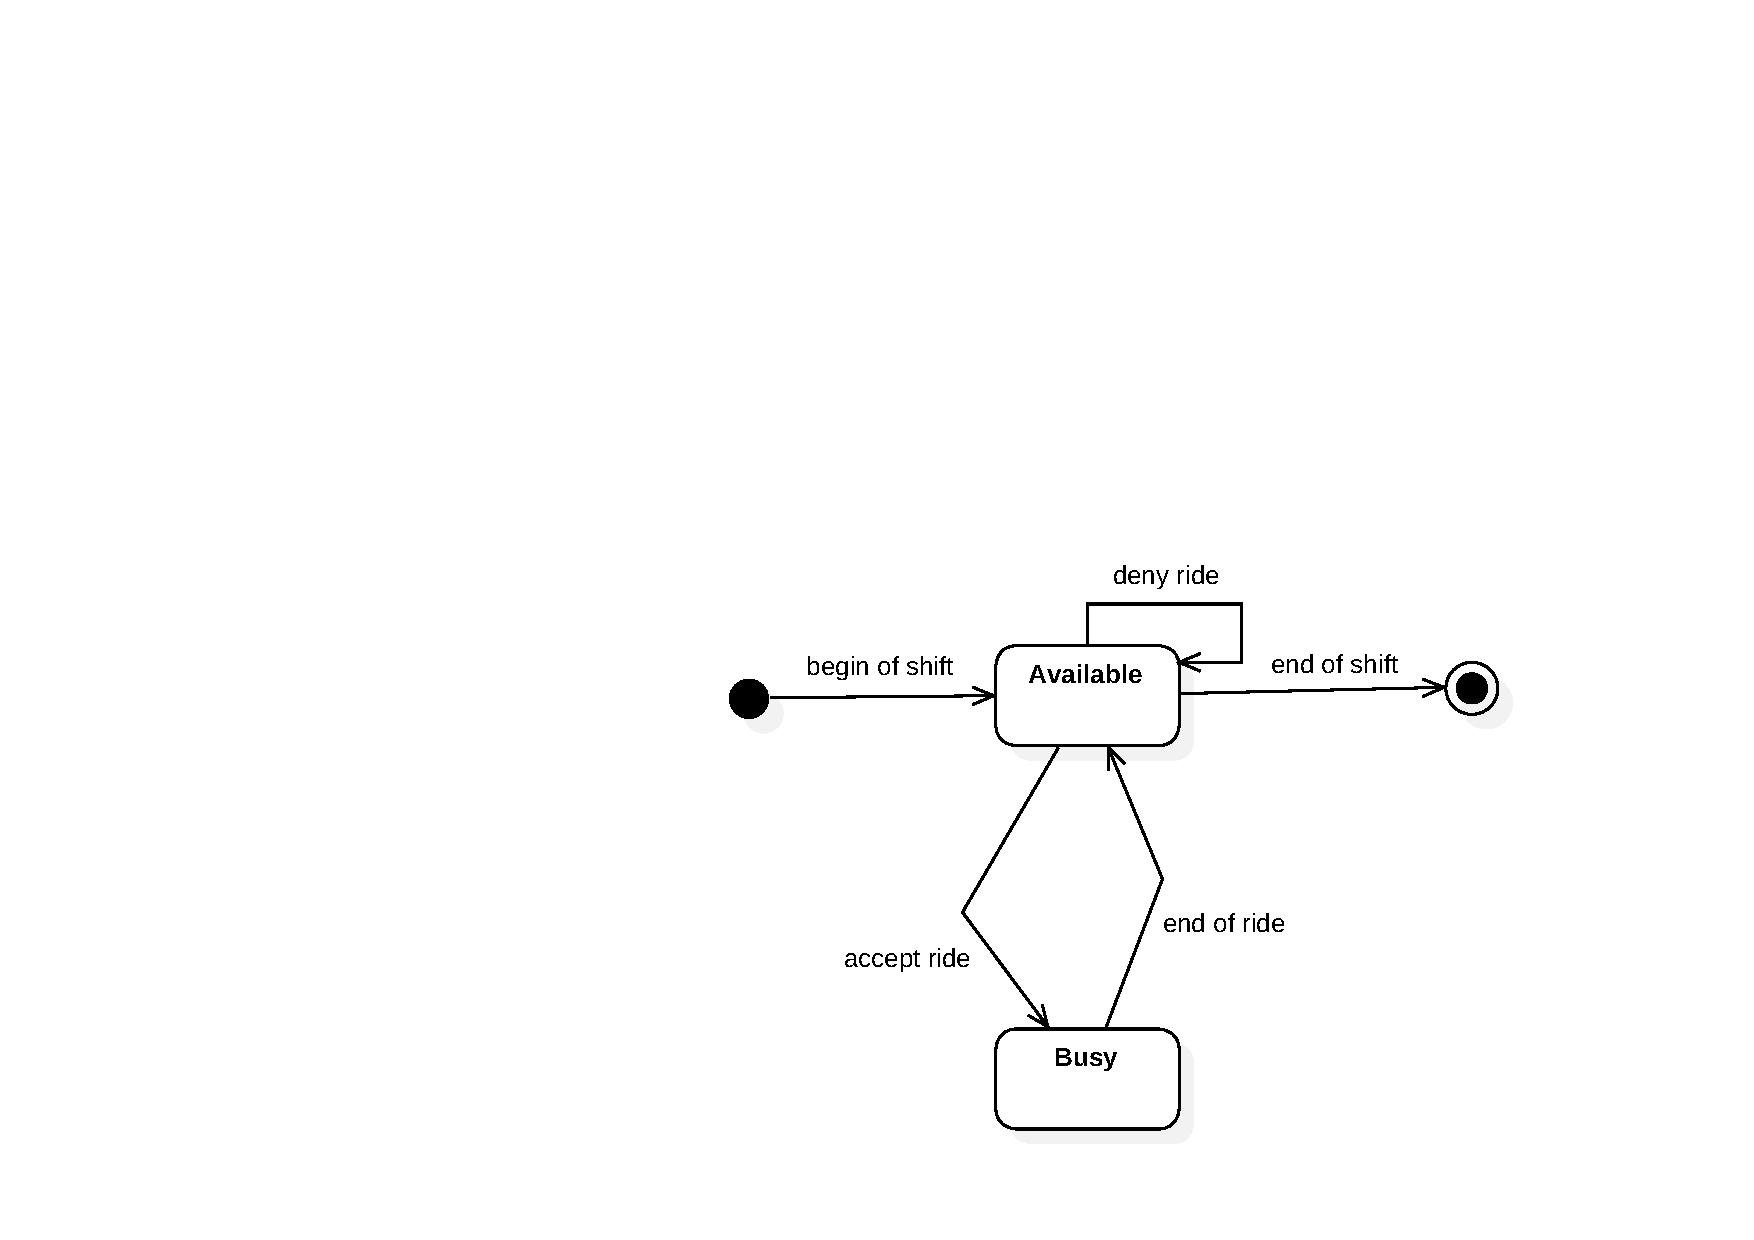
\includegraphics[width=0.7\textwidth]{diagrams/statechart_taxidriver.pdf}
	\caption{Statechart of the possible statuses of a taxi driver.}
	\label{fig:statechart_taxidriver}
	\end{center}
\end{figure}

The response sequence associated with this functionality is shown in~\autoref{fig:taxi_availability}.
\begin{figure}
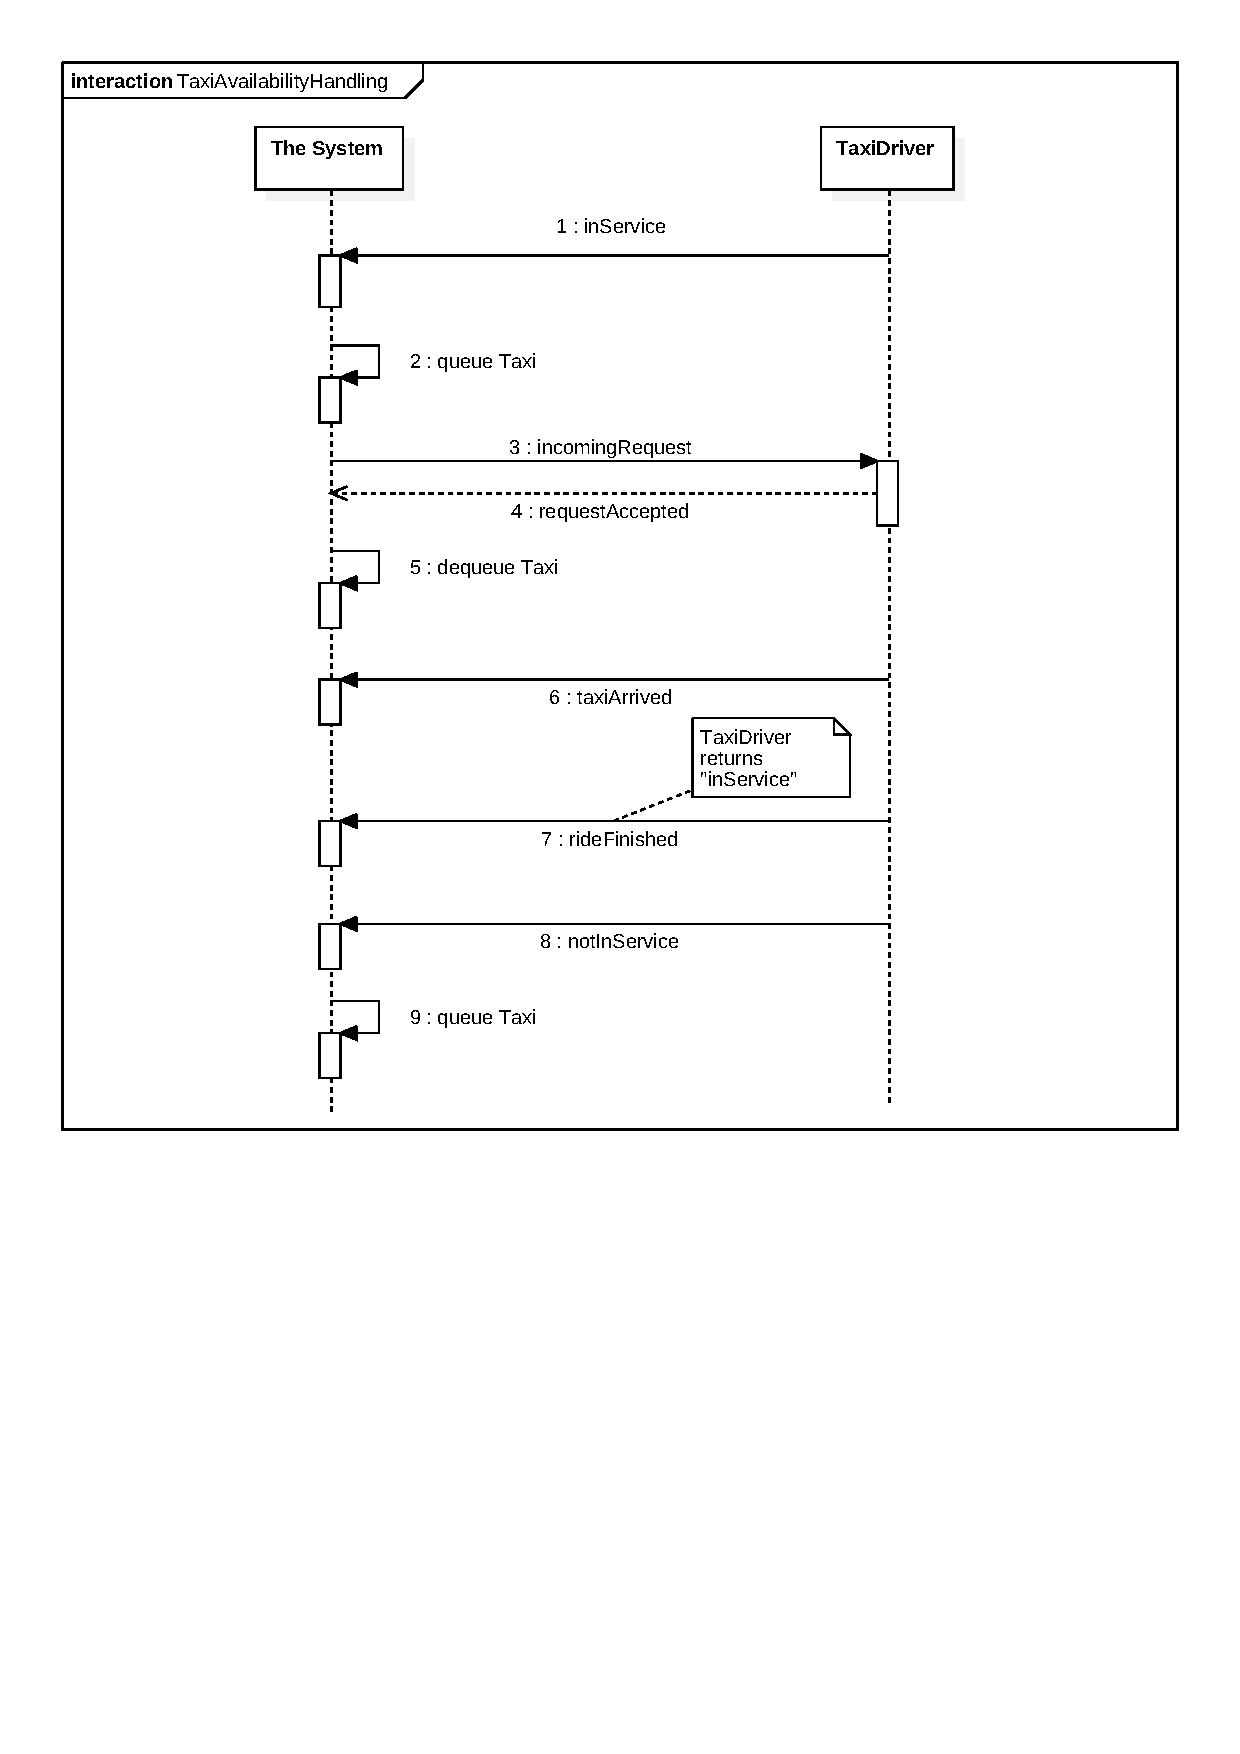
\includegraphics[width=\textwidth]{diagrams/taxi_availability_handling.pdf}
\caption{Sequence diagram of an accepted taxi call.}
\label{fig:taxi_availability}
\end{figure}

\subsubsection{Associated functional requirements}
\begin{enumerate}
\item The system gets the taxi GPS data.
\item The mobile app has to offer to the taxi driver the ``change status'' function and the ``ride complete'' function.
\item The system inserts the taxi in the right queue and changes it if the taxi changes area.
\item For every new request, the system chooses the taxi driver on the top of the queue.
\item The system manages the queues using the FIFO policy.
\item When busy, the taxi driver is presented by the mobile application with the option to end the ride.
\item When the taxi driver ends the ride, he or she is marked as available and gets re-inserted in the taxi queue of the taxi zone where he or she is located.
\item If the taxi driver refuses a ride, he or she is automatically reinserted at the bottom of the queue for his zone.
\item If a taxi driver in ``in service'' state goes out of a taxi zone and enters into another taxi zone, his status is preserved. He is removed from the old taxi zone queue and inserted at the bottom of the new taxi zone queue.
\item If a taxi driver in ``in service'' state goes out of any taxi zone, the system marks him automatically as ``out of service''. When the taxi driver re-enters, he or she may manually change back his status.
\end{enumerate}
